A compartmentalized program consists of isolated compartments with controlled
communication paths between them, as defined by a 
compartmentalization \emph{policy}.
A compartmentalization \emph{mechanism} is responsible for upholding the
isolation and communication rules as described by the \emph{policy}.
A developer has a choice between a plethora of academic and industrial 
mechanisms\footnotemark
proposed to support compartmentalization.
However, mechanisms differ in the threat models they are designed to protect
against, their performance characteristics, the use cases they support, and
their compatibility with existing or upcoming system architectures.
A survey of compartmentalization mechanisms is required to understand the
properties and guarantees of different proposals, and compare their
suitability for compartmentalization use cases.
In this chapter, we will take a deeper dive into a wide range of 
compartmentalization mechanisms and compare them on security and performance
properties.
\footnotetext{In this chapter, the term ``mechanism'' refers to a 
compartmentalization mechanism.}

%%%%% Parts of this background are already discussed in the SecureCells paper.
%%%%% However, we need not repeat this stuff in this section.
% \section{Background on Compartmentalization}

% \begin{itemize}
%       \item Modern software is monolithic, or compartmentalized at a coarse granularity.
%       \item Monolithic software runs all parts of an application in a single address space
%       \item Issues with monolithic software includes:
%             Memory safety bugs can compromise data throughout the address space
%             Control flow hijack/bending allows any code to call any other code
%             Can lead to system calls being called from unexpected code
% \end{itemize}

% In contrast, a compartmentalized program separates logical components of the application
% and isolates them in individual compartments, which implies some degree of separation.
% Isolation restricts which resources each compartment has access to, in order to prevent
% one or more of the above attack vectors.

% Compartments are logical, and not necessarily linked to code. 
% For example, compartments for a browser can include the JIT compiler, the runtime and the
% untrusted sandbox code. 
% While these are isolated, they may have access to the same code, including libraries like
% libc.
% Additionally, there might be one or more sandboxes which are instances of the same module,
% for example, and thereby share exactly the same code regions. 
% However, they would need to have separate data regions or some isolated contexts.
% All of this is to say that we should not make a 1:1 link between code and compartment.

% The aim of this section is to provide background of compartmentalization as a software design principle to provide enhanced security. 
% This section will explain the terminology of "monolithic" and "compartmentalized" programs. 
% This section will also describe the attacker model for compartmentalization and what attacks can be prevented.


%%%%%%%%%%%%%%%%%%%%%%%%%%%%%%%%
\section{Description of use cases and threats}
\label{sec:compreview:usecases}
%%%%%%%%%%%%%%%%%%%%%%%%%%%%%%%%
In this section, we introduce some characteristic use cases for 
compartmentalization, and 
describe some typical attacker models.
These examples will allow us to compare the mechanisms described later.

%-------------------------------
\subsection{Hierarchical trust} 
\label{sec:compreview:usecases:hierarchical}
%-------------------------------
Let us consider a system with hierarchical notions of trust.
In \autoref{sec:seccells:reqs}, we have already encountered the example of
a browser running untrusted code from a web application.
In this application, the JIT engine creates and orchestrates execution of
the sandboxed code.
The JIT engine has access to the WebApp's code and data region, implying
a hierarchical trust relation ---
the WebApp must trust the Engine to correctly generate code and modify
its data.
Despite this hierarchical trust relationship, 
the Engine's permissions (\Code{rw}) to the WebApp's code is not a
superset of the WebApp's (\Code{rx}).
While the Engine's code is separate from the WebApps, the Engine might allow
the WebApp to directly execute specific shared code from 
libraries (say \Code{memcpy}).
The Engine's OS resources must also be isolated and inaccessible by the
WebApp.
The Engine can ensure that the WebApp code contains no syscalls and interpose
every request to OS resources by the WebApp, or install system call filters
which properly restrict syscalls by the WebApp.
Since the system call interface of modern OS kernels like Linux can be used to 
bypass intra address-space compartmentalization~\cite{ConnorMSS20}, we must
assume that every mechanism below is adapted to run with a kernel which
properly isolates OS resources for each compartment (for example, as proposed 
by Schrammel~et.~al.~\cite{schrammel2022jenny}).
\atri{systems restricted to a single trusted/untrusted compartment won't work}
\atri{systems without system call filtering will fail (does ERIM have filtering?)}
\atri{systems where the kernel cannot identify the caller will fail 
      (does donky prevent OS confused deputy, or allow OS to identify caller?)}
\atri{Systems with hierarchical trust, where superset relation is needed will fail}
\atri{CODOMs' where APL grants full permission for a domain's regions will fail}
\atri{Code = Domain, like CODOMs, will bar cross-compartment code sharing}

Adding to the example from \autoref{sec:seccells:reqs}, consider that the
Engine is sandboxing more than one WebApp from different sources.
The WebApps do not trust each other, and must be isolated from each other.
Each WebApp's memory regions and OS resources.
Further, the WebApps should not be able to directly call each other.
Any interaction between WebApps should pass through the Engine.
\atri{Cross-compartment calling restrictions (if callee can ident itself and caller)}

Common threat models for this browser setup would be to assume a buggy Engine
which either
\begin{inparaenum}[\itshape i\upshape)]
      \item generate an arbitrary read or write primitive in the code generated
            for a WebApp, or 
      \item generate arbitrary attacker controlled code for a WebApp.
\end{inparaenum}
Compartmentalization must, nonetheless, protect the Engine and other WebApp 
from a malicious WebApp which exploits the buggy Engine's code generation.
\atri{How many systems break with arbitrary code exec}

%-------------------------------
\subsection{Mutual distrust} 
\label{sec:compreview:usecases:distrust}
%-------------------------------
A workload similar to \Code{memcached} described in 
\autoref{sec:seccells:evaluation:memcached} can have mutual distrust
between directly communicating compartments.
For this section, we assume that the server's data store (Store) compartment
compartment distrusts the server's networking (Network) compartment and
vice versa.
We assume that a malicious attacker who compromises the Network compartment
can try to attack the Store by calling the Store with a malicious register
context.
For example, the attacker Network can use a malicious stack pointer register 
in order to trick the Store to use a wrong region of memory as its stack.
The Network attacker might try to write one of its data regions with a malicious
stack state and point the Store's stack pointer to this region.
In this attack, the Network wants to use the fake stack state to influence the
Store to compromise its own state or the in-memory database.
Further, the Network attacker would need to share the region hosting the fake
stack with the Store, either beforehand or by dynamically passing its 
permissions before calling into the Store.
In a generalized attack, the malicious register may be any register, not
only the stack pointer.
\atri{CHERI can fail the malicious rsp attack/malicious pointer register attack}.
\atri{Systems requiring hierarchical trust will fail.}
\atri{CODOMs' where APL grants full permission for a domain's regions will fail}

In the case of mutual distrust, compartments must use static threading 
and maintain their own context state.
Particularly, the callee on a cross-compartment call must be able to 
restore a clean, trusted register state before processing the incoming request.
Likewise, the caller must be able to restore its own state when the callee
returns control.
\atri{Systems mandating migrating threading will fail}

%-------------------------------
\subsection{Trusting but wary}
\label{sec:compreview:usecases:wary}
%-------------------------------
A workload such as the network function (NFV) pipeline described in 
\autoref{sec:seccells:reqs} might be developed within a more trusted
ecosystem, and have stronger trust relations between compartments.
Let us again consider a pipeline with multiple stages, each of which
is isolated within a separate compartment.
Data packets get moved between pipeline stages as each stage of the
pipeline executes.
The main goals for the pipeline would be to 
\begin{inparaenum}[\itshape i\upshape)]
      \item prevent bugs in one stage from corrupting a separate stage, 
      \item maintain high packet processing rates in order to satisfy
            the network's line rate, and
      \item maintain high availability, where crashes in parts of the
            pipeline are handled gracefully and with minimal downtime.  
\end{inparaenum}
\atri{Fast compartment switching}
\atri{Fast zero copy data movement}
\atri{kernel needs to be able to identify faulting compartment}

Another popular use case is library compartmentalization, where shared
libraries within an application can be isolated within compartments.
Shared libraries, which are often community developed, feature prominently
in applications but can have bugs which compromise the rest of the
application.
Shared libraries can generally be trusted to not be malicious, but can
have bugs. 
Therefore, the compartmentalization policy can require lighter isolation
rules for shared libraries.
Function calls between libraries can also happen at a high frequency in
applications, so low overhead for switching is required.


%%%%%%%%%%%%%%%%%%%%%%%%%%%%%%%%
\section{Properties}
\label{sec:compreview:properties}
%%%%%%%%%%%%%%%%%%%%%%%%%%%%%%%%

In this section, we describe some of the possible guarantees or protections
that compartmentalization mechanisms can provide.
We will also describe the common operations for compartmentalized programs,
which will allow us to explore the performance potential of different
mechanisms.

%-------------------------------
\subsection{Security Properties}
%-------------------------------
Compartmentalization mechanisms aim to provide mitigations for applications
where one or more compartments have been compromised, specifically opposing
further corruption of remaining compartments or the rest of the system.
As described in \autoref{sec:compreview:usecases:hierarchical}, common threat
models assume that a compromised compartment either gives an attacker arbitrary
memory pointer dereference or arbitrary code execution as that compartment.
In this section, we describe possible security properties and how mechanisms
might provide these properties.
These security properties roughly fall into two categories, those that
perform access control to restrict access to resources and reduce
compartment privileges, and those that secure compartment interfaces
which remain the primary attack vector for inter-compartment fault propagation.
We must assume compartments which harden their interface against attacks
which can be triggered through maliciously crafted arguments, as no
mechanism can fully protect an improperly compartmentalized program.

\atri{We can expand greatly on the consequences of lacking security properties
in this section}
\atri{Me might want to make these shortcomings concrete through examples of
actual attacks}

Compartmentalization prevents direct cross-compartment memory access, by 
defining separate memory address spaces for compartments or by 
enforcing per-compartment access rights for intra-address space compartments.
Mechanisms implement access control through variations of page table entries,
segments, permission tables, protection keys or memory capabilities.
Therefore, a compromised compartment cannot directly leak or corrupt a 
different compartment's memory.
Memory access control can also be used for access control to memory-mapped
I/O.

Memory access control must extend to code fetch besides data read/write
accesses.
Modern programming languages rely on code pointers stored in memory or
registers, and indirect calls and returns which use code pointers.
Without access control on code fetch, a victim compartment might be fooled 
into executing code for a different compartment by merely corrupting a
code pointer used during the victim's execution. 
Malicious code injection can be mitigated with permission checks on the
code fetch paths.

Compartmentalization also controls access to system resources.
Mechanisms can separate namespaces for system resource handlers between
compartments, introduce an interposing layer on system calls or 
implement compartment-aware system call filtering.
Separate namespaces prevent compartments from naming other compartments'
resources (e.g., each process has independent file descriptor tables).
System call interposition or filtering can both prevent compartments from
using some system calls or use syscalls with malicious arguments.
For using system call filtering, the mechanism must enable the kernel to
definitively identify the calling compartment.

When compartments communicate, the inter-compartment calling interface 
represents the primary attack vector for a compartment. 
A minimal requirement is that control flow for cross-compartment calls
must enter a compartment at legal entry points.
Failing this, attackers might be able to mount 
return-oriented programming (ROP)-like attacks which leverage unintended
code sequences to bypass compartmentalization guarantees.
Fixed entry points are also vital to implement call gates, which enable
compartments to implement vital checks at inter-compartment interfaces.
We describe a couple of these checks next.

Compartmentalization should limit which compartments are allowed which other
compartments, as an application of least privilege. 
A sandboxing engine could require, for example, that calls between sandboxes
are interposed by the engine.
To implement this check, mechanisms might track allowed caller-callee 
compartment pairs, and validate each cross-compartment call.
Alternatively, mechanisms can allow compartments to validate their own
callers as part of the call gate.
For the latter, a callee must be able to irrevocably identify itself and its 
caller.

When compartments do not trust each other, a compartmentalization mechanism
must enable compartments to maintain their own contexts (static threading).
Without static threading (migrating threading), the register context following
an inter-compartment call may be malicious.
For example, the stack pointer register could point to a attacker-crafted
malicious stack.
Mechanisms might themselves implement secure context switching at compartment
boundaries, or enable compartments to perform the context switch as part of
call gates.
In the latter case, compartments should be able to fetch their register context
securely without trust on any registers passed after the compartment switch.
Compartments must be able to locate a private state store and
restore context from it.
To locate its private state store, a compartment might need a way to uniquely
and securely identify itself. 

Compartments pass arguments for inter-compartment calls by value, through 
registers, or by reference, through memory.
Data passed through memory might use shared memory buffers, be copied between
private buffers by a privileged entity like the OS kernel, or be passed without
copying if the caller can grant permission to the existing location of the data
in memory to the callee.
The third option, called zero-copy, is particularly necessary for high-performance
applications.
Passing permissions raises security challenges, which mechanisms can try to 
mitigate with the following properties. 
First, no compartment should be able to unilaterally grant or seize permission to 
data to or from another compartment respectively.
If a compartment can unilaterally seize permissions for another compartment's data,
this would trivially break isolation.
A compartment could gain access to, and corrupt, another compartment's private
data.
If a compartment could unilaterally grant permission to another compartment, 
compartments could mount confused deputy attacks where the target compartment may
be tricked into using attacker-crafted data whose permissions were injected into
the target by the attacker.
Particularly, this vector could make inter-compartment code injection trivial.
A secure permission transfer should employ a handshake between the source and
target compartments, who agree to mutually transfer permissions.

\begin{figure}
      \centering
      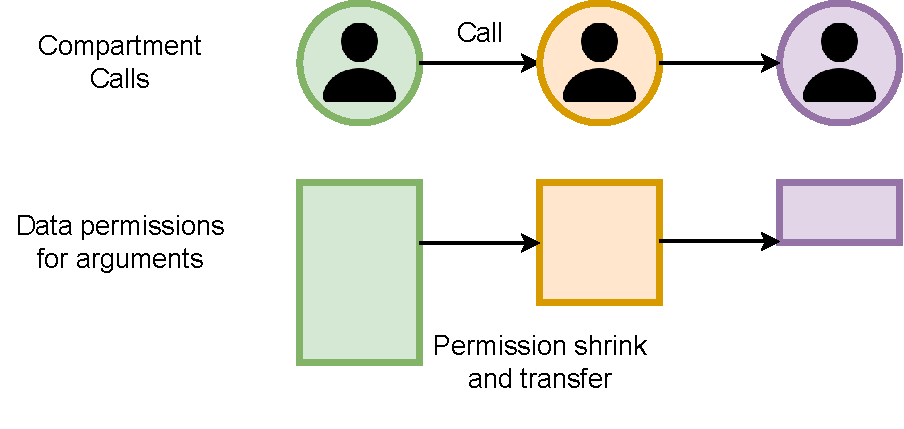
\includegraphics[width=0.75\linewidth]{media/compreview/permission_shrink_grant.pdf}
      \caption[Argument passing by reference between compartments.]
              {Argument passing by reference between compartments, showing a nested call
              where the callers spatially shrink the argument's region and pass permission
              to the next callee. For example, stages in a networking pipeline progressively
              removing each layer of protocol headers.}
      \label{fig:compreview:permshrink}
\end{figure}
Additional properties are desirable when passing
permissions between compartments - revocation and shrinking permissions.
A compartment should be able to selectively transfer permissions for a 
some, not all, of its memory regions.
A common usage pattern is synchronous permission passing, where a caller
compartment intends to transfer permission to arguments to the callee for the
duration of the callee's execution as a form of temporal least privilege.
A corollary is that the callee should no longer have access to the granted
permissions once the callee returns.
Since the caller may not trust the callee to surrender permissions correctly, 
mechanisms can support revocation to allow the caller to revoke the previously
granted permissions when the callee returns.
During nested compartment calls, the callee for the first call might want to pass
permission to a subset of its arguments to the callee for the second call.
We illustrate this situation in \autoref{fig:compreview:permshrink}.
A mechanism which supports this paradigm securely should allow a compartment to
shrink permissions for a region to create permissions for a smaller region
which can be transferred during the second call. 

When an application has concurrent access to writable data regions shared 
between concurrently executing compartments, data races can emerge due to
improperly synchronized access to shared data.
Attackers can exploit such bugs to compromise interfaces, as described for
example in \autoref{ch:midas}.
To mitigate bugs from shared access to data, a mechanism may temporarily provide
compartments exclusive access to otherwise shared data.

%-------------------------------
\subsection{Performance Properties}
%-------------------------------
The performance of a compartmentalized program depends on the cost of
a mechanism's checks and protections, and on the frequency at which these
overheads are encountered.
In this section, we will generally describe the operations required to
support compartmentalization, explain why they are required and their
frequency of occurence. 
This information will allow us to compare the performance characteristics
of compartmentalized applications across different mechanisms.

First, compartmentalization requires access control to resources, particularly
to memory and to OS resources.
Memory is accessed during instruction fetch and for load and store instructions
at nanosecond scale.
Access control to memory is required for all instruction fetches, and for
loads and stores which account for roughly $35\%$ of retired instructions
for SPEC-int benchmarks on average~\cite{LimayeA18}.
A modern desktop or server processor core runs at 2-4GHz clock speed, and
retires more than 1 instruction per cycle on average, which requires
multiple access control operations per cycle.
A mechanism must also be able to scale with application dataset sizes, as
modern applications use gigabytes to terabytes of memory.
Large datasets stress near-core translation or protection caches, such as
the translation lookaside buffer (TLB) on commercial cores.
Mechanisms which rely on TLBs or similar structures might inherit the
scaling limitations of these structures.
Programs access OS resources, generally requiring a system call, at
relatively relaxed time frames.
While more traditional desktop workloads require system calls at 
millisecond-scale, more high-performance server workloads including the
virtualized network function described in 
\autoref{sec:compreview:usecases:wary} may require system calls to access
the network at microsecond scale.

Second, compartments need to communicate with cross-compartment calls.
Typically, mechanisms implement cross-compartment calls as one hardware
core switching from executing the caller compartment to the callee.
Compartment switching is less frequent compared to access control, happening
at sub-microsecond to millisecond timescales.
For example, unmodified Firefox compartmentalizes at a 
coarse granularity, putting individual tabs in separate processes.
Unmodified Firefox is limited to coarse grained compartments due to the high
micro-second scale cost incurred for inter-compartment calls between
processes.
However, we measured that a finely-compartmentalized Firefox switches between
compartments every 750 instructions on average, 
when compartmentalized with every library occupying a separate compartment.
On a modern processor, 750 instructions executes in less than a microsecond.
Cross-compartment calls must also move data as arguments for the call.
Mechanisms might enable data movement through copying, use of shared memory
between the caller and callee, or by transferring permission for the
data regions holding arguments.
Practically, the cost of compartment switching and data movement informs the 
security-performance tradeoff, 
with lower overhead mechanisms allowing applications to implement
finer-grained compartmentalization while maintaining the same performance.
High-performance software requiring 
compartmentalization~\cite{HwangRW14,MartinsAROHBH14,RamCCR13,HondaHLR15}
relies on unoptimal designs like pinning compartments to cores to skip the
cost of switching compartments on a core and reliance on memory shared between
all compartments to prevent data movement between compartments.
Core pinning wastes core time, as each core typically does not need the same
amount of execution. 
When virtualized network functions are pinned to cores, cores executing stages
with lesser computation must wait for cores executing longer stages.
Memory shared between all stages removes some of the benefit of 
compartmentalization, as a corrupted stage can also corrupt data being 
processed by other stages.

%-------------------------------
\subsection{Usability Properties}
%-------------------------------
Compartmentalization mechanisms optimize for different objectives, and vary
widely in design.
Consequently, mechanisms offer different degrees of usability to application
developers.
Ideally, mechanisms aim to be generic and widely applicable, able to support
a wide array of different use cases allowing varied developers to 
benefit from compartmentalization for their applications.
Mechanisms would also ideally allow compartmentalization with minimal developer
effort, through compiler-based automation.

Mechanisms need to be flexible, supporting different policies.
We have discussed use cases with different trust relationships in 
\autoref{sec:compreview:usecases}.
Mechanisms which optimize for sandboxing, for example, might assume
a hierarchy of trust with the sandboxing runtime being most trusted
and sandboxes being untrusted.
A mechanism which only allows hierarchical compartments, however,
will not be able to support relations with mutual distrust between
compartments.
Flexibility also applies to inter-compartment calls, and to the requisite
control or data flows.
Applications might require standard call-and-return control flow,
nested compartment calls, or asymmetric control flow without returns.
When transferring data between compartments, mechanisms should allow
fine-grained spatial definition of data transferred.
Mechanisms which transfer data at fixed granularities, for example a
4 kilobyte page, would be unoptimal.

A mechanism should also integrate with existing and future software and
hardware systems, i.e., maximize compatibility.
Backward compatibility, for example, allows the plethora of existing systems
to use the mechanism with less effort compared to a 
mechanism with a clean-slate design.
As a trade-off, a backward compatible mechanism might inherit shortcomings
of existing mechanisms and may not be usable on newer systems.
In contrast, a forward compatible mechanism would be designed for working
with upcoming or future systems rather than existing ones.

Mechanisms which can automatically compartmentalize existing applications
benefit developers immensely.
Compartmentalization requires principled design of the isolation policy,
and generally requires invasive changes to port over existing monolithic
applications.
As complex applications scale to millions of lines of code,
principled compartmentalization often becomes too expensive.
Automated compartmentalization techniques generally implement weaker
security guarantees compared to manual, principled compartmentalization,
but greatly reduces the cost of adding compartmentalization.
In many cases, automated compartmentalization may be the only 
cost-feasible solution, and the weaker isolation provided is still
safer than monolithic applications.

%%%%%%%%%%%%%%%%%%%%%%%%%%%%%%%%
% Introducing the surveyed mechanisms
\section{Compartmentalization Mechanisms}
\label{sec:compreview:mechanisms}
%%%%%%%%%%%%%%%%%%%%%%%%%%%%%%%%

To understand and compare mechanisms, we first need to understand each 
mechanism, and understand their model for compartmentalization.
In this section, we will describe relevant compartmentalization mechanisms
and summarize their key features.
We will also try to explore their abstractions and isolation model,
and illustrate what compartmentalized programs look like under that model.
Finally, we will try to illustrate how a browser 
(described in \autoref{sec:compreview:usecases:hierarchical}) is 
compartmentalized with each mechanism to protect the JIT engine from
untrusted web application code.

%-------------------------------
\subsection{Process-based compartmentalization}
%-------------------------------

The traditional abstraction of isolation is based on processes.
We will describe process-based compartmentalization in UNIX-like OSs
(particularly Linux), 
though the concepts generalize to other OS kernels.

% Context about how processes emerged
The process abstraction was introduced to isolate programs running on 
multi-user machines.
Each process has an isolated memory space (architecturally-defined virtual memory)
and individual OS resources, such as file descriptors, I/O handles or capabilities.
The OS kernel time-multiplexes processes onto one or more processing cores.
A process can have one or more kernel threads, corresponding to independent threads
of execution, but sharing the same address space and OS resources.
Everything within a process shares the same permissions to access its memory and
its OS resources, including the program's executable, libraries, and loaded modules.

% Explain how processes allow compartmentalization
To compartmentalize a program, that program needs to isolate each compartment in
a separate process.
% Isolation part.
Each process will have its own private memory address space, and its own 
OS resources.
One process cannot name a separate process' resources since they each have separate
namespaces, and hence cannot directly access another process' resource.
OS resources require an open-like step, ensuring that each process in the program
only accesses allowed resources.
Processes cannot arbitrarily gain capabilities.
% Communication part
Processes can, additionally, share memory and specific OS resources for 
communication.
Shared memory must be set up with explicit system calls, and are subject to 
syscall filtering.
The generated code region can be shared between the JIT and sandboxes, along
with code sections for shared libraries.
Processes can also communicate using inter-process communication (IPC) system 
calls (like sendmsg/recvmsg).
A remote (cross-process) procedure call typically consists of serialization of
arguments into a buffer, sending the buffer across using a system call,
and then deserialization of the arguments on the receiving side followed by
the requisite processing based on the arguments.
As we will show later, the cost of inter-process switching contributes a great
deal to the expensive nature of compartmentalization with processes.

% Explain how processes compartmentalize a browser
A browser can be compartmentalized using processes by isolating sensitive
components in separate compartments each of which runs in a separate process.
For example, the browser JIT Engine can occupy one process and each sandbox
can be assigned a separate process.
Microsoft's ChakraCore JavaScript engine~\cite{ChakraCore}, for example, 
used such an architecture to isolate itself from untrusted sandboxes.
A shared memory region between the Engine and each sandbox holds the sandbox's
code.
This region is mapped as executable in the sandbox, and writable in the Engine.
The Engine and sandboxes can communicate using the kernel's inter-process 
message passing system calls.
The Chromium web browser further isolated parts of the Engine interacting with
the local system from the other parts interacting with untrusted 
code~\cite{barth2008security}.

%-------------------------------
\subsection{XPC: Architectural support for secure and efficient cross process call}
%-------------------------------

% Context and introduction of XPC
XPC~\cite{DuHXZC19XPC} shares much of the abstractions from the process-based
isolation, but attempts to accelerate inter-process calls, in particular, 
while maintaining the same interface.
Backward compatibility is a major design directive.
Particularly, XPC replaces the system calls used for IPC with hardware 
instructions supported by state machines implementing the same functionality.
XPC aims to reduce the cost of IPC compared to kernel software, 
also eliminating software dispatch and scheduling overheads in the common case.
XPC also focusses on cheap zero-copy data movement between processes,
dedicating a single relay segment for the purpose.

% Explain how XPC allows compartmentalization
A compartmentalized program running under XPC looks essentially identical
to that using processes.
% Isolation part
Just like previously, each process has their own address space and OS 
resources and capabilities.
The XPC hardware engine tracks the page-table pointer and capability pointer
for each process of a compartmentalized program in an \emph{x-entry} held in
an in-memory \emph{X-Entry Table}.
The OS sets up the X-Entry Table during a program launch.
While a process is running, the XPC engine ensures that the hardware uses the
correct page table pointer and capabilities.
% Communication part
XPC accelerates remote procedure calls, introducing the \Code{xcall} and
\Code{xret} instructions to replace \Code{sendmsg}.
On executing \Code{xcall}, the hardware fetches and installs the relevant 
page table pointer and capabilities for the target process, 
and put an entry for the caller on a \emph{Link Stack}.
Executing \Code{xret} allows the callee to return to the caller, and the
hardware engine pops the caller's information and installs it in the
corresponding system registers (including the return address). 
XPC eliminates the OS kernel from inter-compartment calls, relying on the 
hardware to implement traditional kernel functionality.
Additionally, data passed between processes can use the relay segment, which
is a single dedicated segment mapping memory separately from the page tables.

% Explain how XPC compartmentalize a browser
A browser compartmentalized using XPC looks essentially the same as
using UNIX processes. 
The JIT and each sandbox occupy separate processes.
The major change is that IPC system calls are replaced by 
\Code{xcall}/\Code{xret} pairs.

%-------------------------------
\subsection{Light-weight contexts: An OS abstraction for safety and performance}
%-------------------------------
% Context and introduction of lwc
This paper~\cite{LittonVE0BD16} introduces a new eponymous OS abstraction,
Light-weight contexts ($lwC$s),
which are independent units of isolated execution.
Contexts, like processes, have separate memory address spaces, OS resources,
and capabilities.
However, contexts remain part of a single process and share metadata in the 
kernel, resembling kernel threads.
Contexts offer the primary advantage that switching contexts within a process is 
faster than switching processes, or even kernel threads within the same process.
$lwC$ achieves faster switching between contexts by eliminating unnecessary kernel
processing due to the kernel scheduler and resource accounting.

% Explain how lwc allow compartmentalization
% Isolation part
Contexts diverge from the point of calling \Code{lwCreate} which acts like
the \Code{clone} system call, where each resulting context has an 
independent memory address space and OS resource handles.
Like processes, OS resource handles can persist across a \Code{lwCreate}, or be
invalidated in the child.
Further shared resources can be generated using the \Code{lwOverlay} system 
call.
During program setup, numerous contexts may be created, each of which can
perform private setup steps or further restrict their resource rights using
\Code{lwRestrict}.
% Communication part
Execution of contexts resembles processes, merely replacing inter-process system
calls with the faster inter-lwC switches.

% Explain how lwc compartmentalize a browser
A browser compartmentalized using lwC looks essentially the same as
using UNIX processes. 
The JIT and each sandbox occupy separate contexts, instead of processes.
With $lwC$, message passing system calls will be replaced by
\Code{lwSwitch} system calls.

%-------------------------------
\subsection{Mondrian Memory Protection (MMP)}
%-------------------------------
% Context and introduction of MMP
MMP~\cite{WitchelCA02MMP} tackles the challenge of flexible, 
fine-grained intra-address space isolation.
Intra-address space compartmentalization differs from previous mechanisms,
all of which have separate memory address spaces for each compartment.
In contrast, compartments in MMP (and the following mechanisms) all share the
same address space.
Isolation between compartments relies on different 
memory views, i.e., different permissions to the same address for 
different compartments.
Intra-address space compartmentalization can simplify the process of
porting monolithic programs to compartmentalize them, and allow
smaller compartments with fine-grained memory permissions.
Data transfer for intra-address space compartmentalization can be simpler
than with IPC, since addresses remain valid across compartments.

% Explain how MMP allow compartmentalization
% Isolation part
Each compartment in a program compartmentalized under MMP maps to a protection
domain, with an unique \emph{Domain ID}.
The virtual address space is split into a number of segments.
Each compartment has its own permission table which holds per-segment permissions,
essentially allowing the domain to have its own view of permissions to memory.
The permission tables can be configured to allow segments to be private (only one 
domain has permissions), or shared.
MMP also describes different structures for the permissions table in memory, and
the hardware structures to read and cache permissions.
MMP's permissions tables separate permissions from translation, and are
independent of page tables.
Crucially, MMPs permission tables allow segments starting and ending at
word boundaries instead of page boundaries, allowing spatially fine-grained
permissions.
% Communication part
Compartments in MMP can call each other through system calls or traps, 
which also modify the permissions table base pointer register in hardware.
The paper also proposes that hardware can be used to accelerate this switch,
though the mechanism is not clearly explained.
MMP requires call gates to prevent control flow attacks at inter-compartment
boundaries.
Data can also be passed between domains during switching, by marshalling
data into copied buffers.
However, MMP also introduces the concept of zero-copy data passing between
compartments by modifying the permissions to the segments holding passed data.
However, few details on maintaining coherence of on-chip permission buffers 
are discussed.

% Explain how MMP compartmentalize a browser
In MMP, the browser fits in a single address space with separate protection 
domains assigned to the JIT compiler, and for each of the sandboxes.
For each sandbox, the generated code can be assigned a separate segment
which has different permissions for the JIT Engine domain (writable), 
and for the sandbox domain (executable).
Further, transitions between the sandboxes and the JIT engine use protected
calls with call gates which ensure proper checks on these transitions.

%-------------------------------
\subsection{Code-centric Memory Domains (CODOMs)}
%-------------------------------
% Context and introduction of CODOMs
CODOMs~\cite{VilanovaBNEV14} enabled fine-grained intra-address space 
compartmentalization
with a novel architecture where domains are identified by the executing
instruction pointer (hence the "code-centric" name), and with permissions
to data regions determined by the executing domain. 
Essentially, bits of page table entries identify the domain owning that
page.
Executing an instruction from a page tagged with a domain ID equates to
executing as that domain.

% Explain how CODOMs allow compartmentalization
% Isolation part
Domains in CODOMs each have permission to specific pages of memory: 
those tagged with that domain's tag in the corresponding page-table entry.
A domain cannot access data belonging to other domains, except if
explicitly allowed during access protection lists (APLs).
% Communication part
Compartments can communicate with function calls, which implicitly
cause compartment switches when the domain of the target address page
differs from that of the source.
APLs specify the ability of some domains to call other compartment,
as well as for the caller to share their data with the callee.
While APLs allow domains to permanently share data with other domains,
CODOMs also proposes the use of capabilities to temporarily share
permissions to data during cross-compartment calls.

% Explain how CODOMs compartmentalize a browser
Under CODOMs, a browser must have separate pages corresponding to the
JIT engine and for each sandbox. 
Each domain's pages must be correctly tagged in the page table to allow
the domain to be identified by the hardware.
Each sandbox must own the pages holding their code regions, and have
executable permissions in the page tables. 
The JIT engine can generate new code using additional permissions specified
in the APLs, where the engine should be granted write permission to
each sandbox's domain pages.
\atri{note: APLs enable access to all of a domain's stuff. sigh.}

%-------------------------------
\subsection{Intel Memory Protection Keys (MPK)}
%-------------------------------
% Context and introduction of MPK
Memory Protection Keys assign keys to regions of memory, and maintain
a separate set of access permissions for each key.
While previous implementations in PA-RISC, Itanium and POWER-6 rely on 
supervisor managed protection key permissions, Intel's MPK extension
makes permission changes cheap by allowing userspace modification to
permissions.
MPK uses bits of the page table entry to assign each page a 4-bit color key,
and uses permission bits in the per-core PKRU register to control permissions
to each page color.
PKRU permissions can be arbitrarily changed by userspace, using a special
instruction (\Code{wrpkru}).
A software library (libmpk~\cite{ParkLXMK19}), can be used to virtualize 
page colors, allowing for more than 16 page colors.

% Explain how MPK allow compartmentalization
% Isolation part
When executing a compartment, MPK uses permissions in the PKRU register
to enforce additional restrictions on memory access. 
Each core's PKRU register should only have permissions for page colors as
per the compartment executing on that core.
% Communication part
Compartments in MPK can implicitly switch between each other using the 
\Code{wrpkru} instruction to change the core's accessible page colors.
Along with the permission changes, the application can also use 
function calls to implement cross-compartment procedure calls.
Data can be transferred between compartments using shared page colors.
Changing page colors requires page table entry modifications, implying a
system call, and cannot be done as fast as PKRU writes.
MPK lacks call gates, and software must ensure control flow integrity
between compartments.

% Explain how MPK compartmentalize a browser
A browser can be compartmentalized with MPK, with one page color for the JIT
engine and different colors for each of the sandbox regions.
The PTEs for all generated code regions must have writable and executable
permissions, since PTE permissions are also enforced.
During JIT execution, the PKRU register holds writable permissions for the
sandbox code regions.
During sandbox execution, the PKRU register holds executable permissions for 
that sandbox's code region, and no permissions for any non-sandbox regions.

%-------------------------------
\subsection{ERIM: Secure, efficient in-process isolation with protection keys}
%-------------------------------
% Context and introduction of ERIM
ERIM~\cite{ERIMOberwagner19} builds on top of Intel MPK to implement 
strict call gates for compartment switching, mitigating a major
shortcoming with Intel's MPK technology.
Essentially, ERIM limits the existence of instructions which can
modify the PKRU value (\Code{wrpkru} and \Code{xrstor}) to within
software call gates.
However, ERIM must inspect all newly loaded code, including shared
library or module loading, to ensure that new instructions which
modify the PKRU register are not injected.

% Explain how ERIM allow compartmentalization
% Isolation part
ERIM relies on the same set of MPK permissions described above to
isolate compartments.
% Communication part
ERIM's main differentiating feature are its call gates, which should
be the only parts in the program with executable \Code{wrpkru} or
\Code{xrstor} instructions.
The key feature of ERIM's call gates are that \Code{wrpkru} instructions
are immediately followed by a call to trusted code, or by a condition which
checks the value in the PKRU register. 
The latter check allows control flow attacks which try to load invalid
permissions to be immediately detected.

% Explain how ERIM compartmentalize a browser
A browser compartmentalized with ERIM essentially looks the same as with
MPK, with the JIT engine occupying a trusted compartment, and each sandbox
occupying one untrusted compartment. 
Data can be passed through pointers directly, just as with MPK, though 
compartment transitions use ERIM's aforementioned call gates.

%-------------------------------
\subsection{Donky: Domain keys - Efficient in-process isolation for RISC-V and x86}
%-------------------------------
% Context and introduction of Donky
Donky~\cite{SchrammelWSS0MG20Donky} aims to retain MPK's primary 
performance advantage, by allowing changing memory views in userspace, 
while mitigating its main weakness, 
where an attacker with arbitrary code execution can immediately bypass
MPK's protections.
Donky replaces Intel's PKRU register register with a new DKRU register
which cannot be directly modified by userspace.
Donky effectively introduces a new privilege level within userspace, 
running a special software monitor called the Donky monitor solely 
capable of modifying the DKRU register.
The Donky monitor can be trapped-into by userspace software, enabling the
monitor to serve inter-compartment call requests, among other requests
which modify memory keys.
While Donky's monitor does not run within the supervisor privilege level,
its design of entry-exit through hardware traps and ability to modify
registers not accessible to normal userspace code makes the Donky monitor
similar to previous works of supervisor-mediated compartmentalization.

% Explain how Donky allow compartmentalization
% Isolation part
Compartments in Donky use separate regions of memory, with permission
enforced as per the DKRU register, similar to compartmentalization with
MPK.
These permissions allow memory isolation for compartmentalization.
% Communication part
Compartments can call each other using \Code{dcall}s, essentially trapping
into the monitor which modifies permissions in the DKRU register and
sanitizes register values before dropping into the callee.

% Explain how Donky compartmentalize a browser
A browser compartmentalized with Donky uses separate Donky domains for the 
JIT Engine and for each sandbox, created by calls to the Donky monitor.
The browser can also install \Code{dcall}s between the engine and each
sandbox, but prohibit \Code{dcall}s between sandboxed domains directly.
Each transition between domains using a \Code{dcall} is interposed by the
monitor.
Inter-compartment \Code{dcall}s ensure that compartments are entered at
valid entry points.
Arguments must be passed through either registers, or through shared memory
between domains.

%-------------------------------
\subsection{CHERI: A hybrid capability-system architecture for scalable 
            software compartmentalization}
%-------------------------------
% Context and introduction of CHERI
CHERI~\cite{WoodruffWCMADLNNR14} introduces architectural support for 
memory capabilities.
Architecturally, pointers are replaced by capabilities, which track 
spatial bounds of memory accessible using that capability. 
CHERI compartmentalization~\cite{WatsonWNMACDDGL15} repurposes 
CHERI capabilities, with a customized CheriBSD
kernel to provide intra address-space compartmentalization.
CHERI provides compartmentalization based on the object-capability model, 
where each compartment is represented as an object encapsulating capabilities
for the compartment's code and data regions.
CHERI is drastically different from the previously mentioned mechanisms,
as access permissions for a compartment are not stored in a centralized
permissions table or permissions register.
Instead, CHERI relies on capabilities distributed within a compartment's 
registers and data regions.

% Explain how CHERI allow compartmentalization
% Isolation part
CHERI uses the capabilities to memory to spatially limit the memory regions
accessible to a compartment.
When executing, CHERI requires one or more code and data capabilities. 
For compartmentalization, each compartment encapsulates its code and data
capability within an object, and sealed by an object type capability 
field (\Code{otype}). 
When running as that compartment, those capabilities are installed in CPU
capability registers, allowing the compartment to only access its code and data.
% Communication part
Compartments can call each other using a system call to the CheriBSD kernel,
which securely saves the caller's state to its object, and unseals the
callee's code and data capabilities and installs them in the core's registers 
before dropping into the callee.
Further, CHERI's capabilities greatly simplify passing permission to arguments
during an inter-compartment call.
A CHERI caller can simply pass a capability to the argument in memory during
the call, allowing the callee to use the capability to access the corresponding
memory.
One consequence, which the caller must be careful about, is that the callee can
use any capabilities stored in this argument memory region to further access other
regions of memory.
CHERI compartmentalization, though, lacks a mechanism for revocation,
instead suggesting the use of garbage collectors for eventual revocation.
A key concern for developers using CHERI is the possibility of capabilities
being leaked during inter-compartment calls.

% Explain how CHERI compartmentalize a browser
With CHERI, each of a browser's compartments must be allocated a separate
object encapsulating that compartment's code and data.
The JIT Engine would be an object, and each sandbox will be implemented as
a separate object.
Both the JIT engine and sandboxes must each hold capabilities to the
sandbox's code region.
The JIT engine can use its own capability to a sandbox's code region,
permitting write operations to generate new code for the sandbox.
The sandbox's own capability for this region must only allow executable 
operations.
Finally, the JIT engine can pass temporary capabilities to sandboxes
when they are required to process certain data, including new data packets,
with zero-copy.

%-------------------------------
\subsection{SecureCells: A Secure Compartmentalized Architecture}
%-------------------------------
% Context and introduction of SecureCells
SecureCells~\cite{BhattacharyyaHLGSFP23} introduces a compartmentalization 
mechanism based on hardware
access control to variable-sized regions of memory, hardware tracked
compartment identifiers, a unified permissions table for all compartments,
and unprivileged instructions for securely accelerating common operations.
SecureCells' permissions table stores permissions for each compartment to
each data region.
Further, SecureCells' userspace instructions enable control flow and
zero-copy data movement between compartments with unprivileged instructions.
SecureCells' unprivileged instructions implement hardware checks in order
to prevent privilege escalation.

% Explain how SecureCells allows compartmentalization
% Isolation part
Each compartment in SecureCells is assigned a \secdiv{}, whose accesses
to memory regions are checked with an in-memory permissions table.
Properly configured permissions allow compartments to have private regions
to which on that compartment has permission, and selectively shared regions
with specific other compartments having permission. 
When executing code for a compartment, a core tracks the executing compartment
identifier in a system register, and accordingly presents a view of memory.
% Communication part
Compartments can also interact with unprivileged \Code{SDSwitch} instructions
which atomically  switch to a different compartment and jump to the callee's
entry point.
To aid zero-copy data transfer, SecureCells also includes unprivileged instructions
which move permissions for regions between compartments.

% Explain how SecureCells compartmentalize a browser
A browser compartmentalized with SecureCells will require separate
\secdiv{}s for each sandbox and for the JIT engine.
The permissions table is set up with per-sandbox private regions, to which
only each sandbox and the JIT engine have permission.
The permissions can allow the JIT engine write access and a sandbox
execute access to that sandbox's code region.
The JIT engine can use \Code{SDSwitch} to enter and exit sandboxes.
Compartments must use the \Code{SDEntry} instruction to mark valid entry points
leading to call gates to switch context and check inter-compartment call
arguments.
If arguments are isolated within a memory region, compartments with 
\seccells can also move these arguments between compartments without copying
by transferring permissions.

%%%%%%%%%%%%%%%%%%%%%%%%%%%%%%%%%%%%%%%%%%%%%%%%%%%%%%%%%%%%%%%%%%%%%%%%%%
% Introducing the classification metrics
\section{Comparing Compartmentalization Mechanisms}
\label{sec:compreview:comparison}
%%%%%%%%%%%%%%%%%%%%%%%%%%%%%%%%%%%%%%%%%%%%%%%%%%%%%%%%%%%%%%%%%%%%%%%%%%
In this section, we will compare the mechanisms presented in 
\autoref{sec:compreview:mechanisms} on how well they provide the properties
required for compartmentalization as discussed in 
\autoref{sec:compreview:properties}.
\autoref{tab:compreview:summarytab} summarizes this comparison.

Mechanisms differ in the performance characteristics, based on the 
common latency of their operations.
While the performance comparison in this section focusses on the 
average latency of operations, high-performance datacenter software 
may also be affected by the tail latency~\cite{LiSPG14} of these operations.

% Other properties to be added
% - Return addresses/link stacks

\begin{table}
  \begin{threeparttable}
    \begin{tabular}{l | l | l | l | l | l}
          Mechanism & Threat Model &  Access Control     & Syscall Filtering & Entry Point         & Threading     \\ \midrule
          Process   & A + B + C    &  Data + Instruction & OS-tracked        & OS-tracked          & S             \\
          XPC       & A + B + C    &  Data + Instruction & HW-tracked        & HW-tracked          & S/M\tnote{3}  \\
          $lwC$     & A + B + C    &  Data + Instruction & OS-tracked        & OS-tracked          & S             \\
          MMP       & A + B + C    &  Data + Instruction & OS-tracked        & OS-tracked          & S             \\
          CODOMs    & A            &  Data + Instruction & HW-tracked        & HW-tracked\tnote{2} & S/M\tnote{3}  \\
          MPK       & A            &  Data               & None              & None                & M             \\
          ERIM      & A + B        &  Data               & None\tnote{1}     & SW-enforced         & S/M\tnote{3}  \\
          Donky     & A + B + C    &  Data               & Inbuilt           & Lib-tracked         & S             \\
          CHERI     & A + B + C    &  Data + Instruction & OS-tracked        & OS-tracked          & S             \\
          \seccells & A + B + C    &  Data + Instruction & HW-tracked        & HW-checked          & S/M           \\ 
          \bottomrule
    \end{tabular}
    \begin{tablenotes}
      \item[1] ERIM has limited support for filtering.
      \item[2] CODOMs' entry point restrictions can be weak.
      \item[3] Limited support for static threading.
    \end{tablenotes}
  \end{threeparttable}
  \caption[A comparison of comparmentalization mechanisms (summarized)]
        {
        A comparison of comparmentalization mechanisms (summarized).
        The threat model column uses threat definitions (A/B/C) from 
        \autoref{sec:compreview:comparison:model}.
        The threading model is defined by S = Static, and M = Migrating.
        }
  \label{tab:compreview:summarytab}
\end{table}


\begin{table}
      \ContinuedFloat
      \begin{tabular}{l | l | l | l | l |l}
            Mechanism & Call control & Permission Tx.         & AC Scalability &  Switch (cycles) \\\hline
            Process   & Filtering    & Bilateral              & TLB-stressed   &  $\sim 10^{3}$        \\
            XPC       & Hardware     & Relay segment          & TLB-stressed   &  $\sim 10^{1}$        \\
            $lwC$     & Filtering    & Static, controlled     & TLB-stressed   &  $\sim 10^{3}$        \\
            MMP       & Filtering    & None                   & Scalable       &  $\sim 10^{3}$        \\
            CODOMs    & Hardware     & Static, limited        & TLB-dependent  &  $\sim 10^{1}$        \\
            MPK       & None         & None                   & TLB-dependent  &  $\sim 10^{1}$        \\
            ERIM      & None         & None                   & TLB-dependent  &  $\sim 10^{1}$        \\
            Donky     & Filtering    & None                   & TLB-dependent  &  $\sim 10^{2}$        \\
            CHERI     & Hardware     & Capability, Revocation & Scalable       &  $\sim 10^{2}$        \\
            \seccells & SW-checked   & Bilateral              & Scalable       &  $\sim 10^{1}$        \\
      \end{tabular}                    
      \caption[]
      {
      (cont.) A comparison of comparmentalization mechanisms (summarized).
      ``AC'' = Access Control.
      We report compartment switching latencies as order of magnitude of cycles.
      }
      \label{tab:compreview:summarytab}
\end{table}

%-------------------------------
\subsection{Threat Model}
\label{sec:compreview:comparison:model}
%-------------------------------
All of the mechanisms discussed in this section provide varying levels of 
protection for a compartmentalized application when 
one or more compartments is compromised.
In each mechanism, the underlying OS kernel is part of the trusted computing
base (TCB) and is considered to be correct.
Essentially, the kernel must be designed to support userspace 
compartmentalization, and must not contain system calls or bugs which can
be used to circumvent the restrictions imposed by a mechanism.

The mechanisms being compared are designed to protect against different
threat models, with an attacker possibly being able to access three
main attack vectors.
\begin{itemize}
      \item \textbf{Threat A}:
            A compromised compartment may contain memory corruption bugs 
            allowing an attacker to attempt to memory regions to which the 
            compartment has no access.
            In this threat model, we assume that the attacker can craft and
            attempt to dereference arbitrary pointers.
      \item \textbf{Threat B}:
            An attacker might control a corrupted compartment with a 
            control-flow hijack.
            In this threat model, we assume that the attacker can use 
            call/return instructions to try to hijack control flow. 
            With return-oriented programming~\cite{Shacham07,vander17} attacks,
            an attacker can leverage hijacked control flow to also dereference
            arbitrary pointers.
      \item \textbf{Threat C}:
            Bugs in a compromised compartment might allow an attacker to modify
            its code, leading to arbitrary code execution.
            In this attack model, we assume that the attacker can inject and 
            execute arbitrary code sequences within a compartment, including 
            possibly privileged instructions.
\end{itemize}

In \autoref{tab:compreview:summarytab}, the ``Threat Model'' column summarizes
the threat models mitigated by each mechanism.
All of the mechanisms surveyed uses access control to protect against the 
first threat model.
CODOMs and MPK fail to protect against both of the latter threats.
With CODOMs, an attacker with control-flow hijack can use indirect calls to
directly jump between compartments, bypassing call gates.
With MPK, an attacker can use ROP attacks to use \Code{wrpkru} instructions
in unintended sequences, or use misuse unaligned code addresses decoding to
\Code{wrpkru} or \Code{xrstor} instructions, to elevate its permissions to
all page colors.
Additionally, ERIM can be defeated by an attacker with arbitrary code 
injection (Threat C). 
ERIM relies on controlling the presence of \Code{wrpkru} or \Code{xrstor}
instructions, which arbitrary code injection bypasses.

%-------------------------------
\subsection{Access Control Permissions}
%-------------------------------
As discussed in \autoref{sec:compreview:properties}, mechanisms need to 
implement access control to memory to isolate compartments.
Access control checks should apply to compartments for both code and data
accesses.

Mechanisms (processes, XPC, $lwC$) implementing per-compartment memory 
virtual address spaces with separate page tables implements checks on both 
data and code based on page-table entry permission bits.
Protection-key based mechanisms, however, limit their checks to only
data accesses.
CODOMs links code addresses to compartments, preventing a compartment from
executing another compartment's code, implicitly implementing code
access control.
CHERI's compartment objects encapsulate both data and code capabilities,
with the former being used for loads and stores, and the latter being 
necessary for instruction fetch.
MMP's permission tables specify read-write, read-only and read-execute
combinations of permissions, thereby controlling data and code accesses.
\seccells' \ptable structure encodes independent read/write/execute
permission bits.
The access control permissions are summarized in the ``Access Control''
column in \autoref{tab:compreview:summarytab}.

%-------------------------------
\subsection{Access Control for OS resources}
%-------------------------------
Compartmentalization requires isolation and access control for OS resources.
In this section, we will discuss whether, and to what extent, mechanisms 
support this requirement.
We will assume that the OS system call interface does not trivially allow
access to other compartments' memory, focussing mainly on other OS resources
like files and open handles.
System call filtering support is summarized in the ``Syscall filtering''
column in \autoref{tab:compreview:summarytab}.

Some mechanisms include explicit system call filtering.
Unprivileged userspace in Donky is not allowed to execute system calls,
which are restricted to Donky's privileged library (DonkyLib).
System calls by compartments trap into DonkyLib which can implement
compartment-specific checks in software for system call filtering.
In \autoref{tab:compreview:summarytab}, Donky is labeled as having ``Inbuilt''
support.

Mechanisms which rely on system calls to switch compartments allow
the kernel to explicitly track the executing compartment, and therefore
the caller for system calls.
Existing system call filtering mechanisms can be extended to support
per-compartment filtering with process-based isolation, $lwC$, MMP and
CHERI.
$lwC$ further supports parent contexts to intercept system calls for
their children if the children were created with the \Code{LWC_SYSTRAP}
flag. 
In $lwC$, parent contexts can also perform system calls on behalf of 
children using the \Code{lwSyscall} system call, which is useful for
applications with hierarchical trust between compartments.
These mechanisms are labelled as being ``OS-tracked'' in 
\autoref{tab:compreview:summarytab}.

\seccells, XPC and CODOMs allow the OS to identify the userspace compartment 
using a system call, and can enforce per-compartment system call filtering 
rules using these identifiers.
\seccells tracks the currently executing compartment with the  \sid register,
which gets copied to the \rid register on system calls, allowing the kernel to
determine its caller.
Similarly, CODOMs tracks the executing userspace compartment in the 
\Code{currdom} register, though its behavior during a system call is not
clearly described in the paper.
XPC tracks the executing compartment as the register \Code{x-entry-table-reg}
indexing into the X-entry Table.
These mechanisms are labelled as ``HW-tracked'' in 
\autoref{tab:compreview:summarytab}.

Finally, MPK and ERIM offer no explicit way to track the executing compartment
and no support for inbuilt system call filtering.
With both MPK and ERIM, the state of the PKRU register implicitly encodes the
running compartment.
However, ERIM can enable some form of system call support by marking code pages 
containing system calls in untrusted compartments as non-executable, thereby
trapping into the kernel which can forward a signal to a trusted compartment.
However, this mechanism is not robust, and introduces false signals due
to execution of any other code on a page alongside a system call.
These mechanisms are labelled as being ``None'' in 
\autoref{tab:compreview:summarytab}.

%-------------------------------
\subsection{Inter compartment call gates}
%-------------------------------
\paragraph{Fixed Entry Points}
Compartmentalization requires call gates for calls between untrusted 
compartments.
Implementing call gates require compartments to be able to define
fixed entry points, which are enforced by the mechanism.
At call gates, compartments can execute further protections
like context switching and argument validation.
This protection is summarized in the ``Entry Point'' column.

Process-based isolation, $lwC$, MMP and CHERI use system calls
and rely on the supervisor for switching compartments.
Therefore, the supervisor can ensure fixed entry points for these
mechanisms, and typically also implement a mandatory context switch
to the callee's context.
For processes, the entry points for each compartment are the 
address following system calls for receiving data 
(\Code{recv}-family syscalls for Linux).
For $lwC$, the instruction following \Code{lwCreate} and \Code{lwSwitch}
represent a compartment's entry points.
Similar return points for compartment switching system calls for MMP
and CHERI limit entry into compartments.
These mechanisms are labelled ``OS-tracked'' in 
\autoref{tab:compreview:summarytab}.
Donky's privileged DonkyLib implements functionality similar to OS kernels, 
interjecting inter-compartment calls and enforcing fixed entry points.
Donky is therefore labeled as ``Lib-tracked''.

Compartmentalization can also rely on the mechanism to track entry points for
compartments.
XPC's X-entry table contains a single entry address for each compartment,
allowing the compartment to implement checks following the entry.
CODOMs tracks executable pages containing domain entry points, but only
restricts entry points within a page to a configurable alignment.
CODOMs' restrictions can be bypassed to access unused addresses in
entry pages respecting the alignment constraint.
We label XPC and CODOMs as ``HW-tracked'', though CODOMs' entry point
restrictions can be weak depending on system configuration.

ERIM does not track entry points for compartments, instead securing 
inter-compartment call gates (including the crucial \Code{wrpkru} instruction)
with specific code sequences.
ERIM's code sequences check permissions in the PKRU register in the call
gates following PKRU writes, ensuring that a correct value is written.
However, the paper is not clear how this check is implemented for mutually
distrustful compartment or comparments with dynamically-changing permissions.
ERIM's call gates are classified as ``SW-enforced''.

\seccells relies on a special instruction \Code{SDEntry} to explicitly
mark compartment entry points, with the hardware checking for valid
entry markers following each compartment switch.
Further, the memory region for each \Code{SDEntry} should only be executable
for the specific compartment using that entry point.
The hardware does not track a list of valid entry points, and
malicious compartments are free to specify arbitrary entry points when
using an \Code{SDSwitch}, raising a trap when used maliciously.
Further call gate checks can, of course, follow the entry point.
\seccells is classified as ``HW-checked''

Finally, Intel's MPK is the least secure mechanism surveyed, since the
mechanism contains no specific provision for securing inter-compartment
switches.

\paragraph{Threading Model}
Secure call gates also imply the use of the static threading model, with each
compartment having its own context.
However, migrating threading can accelerate inter-compartment calls when using
a weaker threat model.
This protection is summarized in the ``Threading'' column.

Supervisor mediated switches, in process-based isolation, $lwC$, MMP
and CHERI switch contexts in the supervisor during the inter-compartment
switch, and mandate static threading.
Donky's library, similarly, protects non-argument registers across
a \Code{dcall}.

Meanwhile, mechanisms with hardware-tracked compartment switches
(XPC, CODOMs, MPK, ERIM, \seccells) do not automatically switch register
context, and support migrating threads by default.
Additionally, some of these mechanisms can also support static threading
if the callee compartment can locate and restore its register context 
after a compartment switch without trusting any of its registers, which could
be maliciously controlled by the caller.
In that case, software in the call gate could save the caller's state in the
caller and restore the callee's state after the switch.
However, MPK do support secure call gates, and cannot satisfy this requirement.
Compartments in XPC and CODOMs cannot explicitly identify themselves, but can
rely on context storage in memory regions at fixed, pre-determined offsets 
from entry points.
Code following entry points could use these hard-coded offsets to restore
the callee's state.
However, this design would prevent compartments in XPC from sharing code for
entry points.
ERIM can also use similar context store regions at fixed offsets from 
call gate entry points to implement static threading, though the generic 
case for multiple compartments is not clear from the paper.
Finally, \seccells allows compartments to explicitly read the \sid register
to identify themselves, allowing them to index into a state store and
restore their state, as described in \autoref{sec:seccells:design:softmech}.

\paragraph{Calling restrictions}
Finally, compartmentalization should limit the ability of compartments to 
call other compartments.
Inter-compartment calling restrictions should only allow calls for specific
caller-callee pairs.

System-call filtering rules, for example, can be used to restrict calls
with supervisor-mediated mechanisms like processes, $lwC$, and MMP.
The supervisor can validate whether a caller-callee transition is allowed
based on rules installed at program startup.
While the paper does not describe call filtering, Donky's privileged
library can also validate compartment switches against a pre-specified
allowlist using softare, similar to system-call filtering.

Hardware-checked mechanisms can also be used to validate calls.
XPC maintains a two-dimensional XCALL capability bitmap, which defines
the allowed caller-callee pairs for the call.
CODOMs' access protection list explicitly contains permissions for each
compartment to call other compartments, which is checked by the hardware
on each switch.
Finally, compartments in CHERI hold capabilities to call other compartments,
which are validated when a compartment runs the \Code{CCall} instruction.
We label each of these mechanisms as ``Hardware'' in 
\autoref{tab:compreview:summarytab}. 

\seccells lacks hardware validation of compartment switches, as switches
to legitimate compartment entry points always succeed.
However, \seccells supports call gates, and allows software to securely
identify the caller-callee pair by reading the \rid and \sid registers
respectively.
A compartment can maintain its own list of permitted callers, and can
refuse to process calls from compartments not on this list.
Therefore, software in call gates can effectively limit permitted
compartment switches in \seccells.

Finally, MPK and ERIM does not support limiting inter-compartment calls.

%-------------------------------
\subsection{Permission transfer}
%-------------------------------
Process-like mechanisms typically communicate via supervisor-based
message passing based on copying data between their own private virtual 
address spaces via kernel buffers.
Processes can traditionally share data regions by mapping shared 
memory files.
However, newer system calls like \Code{vmsplice} allow processes to directly
remap pages from one process into another, when both processes use this
syscall.
Therefore, zero-copy data movement is possible, with bilateral agreement
between the sending and receiving processes.

$lwC$ offers the \Code{lwOverlay} system call which maps resources from
one context into another, overwriting any existing resources at the target
address.
While the compartment receiving access to new data requires a capability
to map the requested data (as an access capability), ensuring that a 
context cannot unilaterally grant itself access to another context's
memory, these capabilities are determined at context creation and are
not dynamically granted.

CHERI controls access to memory based on capabilities, and offers a
convenient system for transferring permissions to arguments during a
cross-compartment call.
A CHERI compartment can pass one or more capabilities to memory holding
arguments to the target compartment during a call, allowing the target to
use the capabilites to access the arguments.
Further, CHERI capabilities can be shrunk, allowing a compartment to
pass on permission for subregions during nested compartment calls.
Finally, compartments can use memory capabilities to further load
capabilities from the memory region permitted by the initial capability.
Therefore, compartments can transfer access capabilities to complex 
data structures by simply transferring the capability for the entry
to the data structure.
For example, the capability to a linked-list's head allows access to
all of the link list through capabilities to the next node stored in 
each node.
However, CHERI's capability-based access control raises the spectre of
unintended capability leakage through complex data structures holding 
further capabilities.
CHERI also supports revocation of capabilities, though systems requiring
frequent capability revocation may suffer from high overheads.

\seccells allows compartments to transfer permissions for memory 
regions (\cell{}s) through a pair of \scgrant-\screcv instructions.
The former instruction is used by the sending compartment to stage a 
permission grant whereas the latter instruction is used by the receiving
compartment to accept staged permissions.
Therefore, permission transfers in \seccells requires bilateral involvement,
making this mechanism secure.
However, compartments cannot easily shrink the region of permissions
for transmitting to another compartment during a nested compartment call,
limiting its flexibility.
\seccells' memory regions also lack the concept of ownership, and
permissions once granted cannot be revoked.

Some mechanisms offer limited or no support for zero-copy data
movement between compartments.
MMP describes zero-copy data movement from the kernel to userspace
by dynamically mapping received network buffers into userspace
during a \Code{read} system call, but does not describe a way to
move data between compartments without copying.
Similarly, MPK and ERIM does not have any checks on permission 
transfers betweek compartments as each compartment can specify its 
own permissions to data regions.
XPC relies on a single relay segment to transfer data between
compartments without copying.
XPC's relay segment has the added benefit that compartments
can shrink the segment before passing the segment forward during
nested compartment calls.
CODOMs allows compartments to share their data with other compartments
by specifying capabilities in the access protection lists (APL).
However, the APLs are static and grant access to all of a compartment's
memory regions to the target compartment.
CODOMs' APL-based permission granting, therefore, does not support 
dynamically moving permissions for small argument buffers between
compartments without copying.
Donky also lacks calls for dynamically moving permissions to regions
between compartments.

%-------------------------------
\subsection{Access Control Performance}
%-------------------------------
Mechanisms perform permission checks for memory access every cycle,
on average.
The performance of modern processors relies on single-cycle permission
checks and address translation for memory access, as these operations
are on the critical path to loading data from the tightly-coupled L1 caches.
As application data working sets have also grown over decades, near-core
caches for storing permissions have been stretched beyond their limit.
Translation Lookaside Buffers (TLBs) on modern architectures can effectively
cache a few thousand translation and protection entries, corresponding to
a TLB reach of a few megabytes of data.
Meanwhile, many modern applications have larger data working sets, causing
thrashing in the TLBs, significantly hurting application 
performance~\cite{0003BOBFP21midgard}.
Compartmentalization can potentially exacerbate this issue, since each
memory region will have different permissions for different compartments,
requiring TLB-like on-chip caches to store even more permission entries
corresponding to different compartments.
In this section, we will compare the potential average access control
performance of different mechanisms, based on whether they require 
permission storage caches near the core which can scale with application
datasets and provide single-cycle permission checks.

Process-based compartmentalization, XPC and $lwC$ all rely on 
page-granularity permissions stored in page table entries in 
per-compartment page tables. 
Each page requires individual page table entries from each compartment's 
page tables in order to express the differing permissions for that page.
The application's permissions will be cached in each core's TLB alongside
translation entries for each page.
Consequently, compartments will divide the TLB capacity between themselves,
leaving each compartment with an effectively smaller TLB capacity.
These mechanisms are most likely to hit TLB reach limits, causing TLB
thrashing.
These mechanisms are labelled as ``TLB-stressed'' in 
\autoref{tab:compreview:summarytab}, as these mechanisms increase the
stress on the TLB.

CODOMs, MPK, ERIM and Donky continue to rely on page table entries (PTEs) 
to store permission metadata.
CODOMs stores each page's owning compartment in the corresponding PTE.
MPK, ERIM and Donky rely on page colors (keys) also stored in PTEs.
While each of these mechanisms rely on page-granular PTEs cached in
TLBs, these mechanisms do not require duplicated PTEs for the same page.
These mechanisms will face TLB reach limits as modern applications do,
but will not worsen the situation.
CODOMs also requires caching for its access protection lists, including
an APL cache for each core.
However, a APL cache can be much smaller than the TLB, as applications
typically deal with more (thousands or millions) data pages than
compartments (10s), and is less likely to encounter scaling limits.
These mechanisms are labelled as ``TLB-dependent'' as these mechanisms
scale with TLBs.

MMP separates protection from translation, relying on two separate permission
storage formats.
MMP's multi-level permissions table (MLPT) resembles the radix trees used for
page tables, with each leaf entry holding the permission for a 4-byte word.
Consequently, MMP's core-side permissions lookaside buffer (PLB) caching
permissions from the MLPT will require 1000x more entries compared to modern
TLBs.
PLBs are build from conventional content addressable memory structures, just
like TLBs, and will hit scaling limits before TLBs.

Two mechanisms store permissions to ranges of memory rather than fixed-size
regions.
MMP proposes a second protection storage format, the Sorted Segment 
Table (SST).
\seccells proposes a protection table (\ptable) structure for permissions.
Both the SST and \ptable store permissions for variable-size ranges of memory.
Consequently, these structures can represent permissions for multi-page regions
with a single entry, reducing the duplication in these tables.
Further, MMP's PLB and \seccells' TLB-like translation cache both require fewer
entries to cache an application's working set's permissions.
Further, range-based memory allows permission caches to scale to large dataset
sizes, since applications typically increase the size of their memory regions
with larger datasets instead of using more regions.
Labelled as ``Scalable''.

CHERI removes the dependence on permission caches, as permissions are encoded
alongside pointers within capabilities.
CHERI's capabilities increase a program's data working set as each pointer
increases from occupying one word (64-bit on 64-bit machines) to two words.
However, capabilities can benefit from the large (64kB or larger) data 
L1 caches on modern machines.
Labelled as ``Scalable''.

Process-based isolation, XPC,  $lwC$, CODOMs, MPK, ERIM and Donky are closely
integrated with modern page-based virtual memory, and will not easily
integrate with future range-based virtual memory architectures.
These systems will suffer from the TLB's scaling limitations for translation,
apart from for protection.
CHERI is agnostic to the translation mechanism, and can move from modern
page-based systems to future range-based systems without any modification.
Finally, MMP and \seccells already dependent on range-based translations,
being better compatible with future systems than modern ones.

%-------------------------------
\subsection{Compartment Switching Performance}
%-------------------------------
Applications demand a widely-varying frequency of compartment switching,
though applications typically tailor their software organization to
fit the compartmentalization mechanism they depend on in order to meet
performance requirements.
Essentially, mechanisms with faster compartment switches can allow
applications to be compartmentalized into smaller compartments, potentially
improving security.

Process-based isolation, $lwC$, MMP depend on traditional supervisor-mediated
compartment switches, costing up to tens of microseconds on each call.
Supervisor-mediated switching potentially incurs the cost of context switches
to and from the supervisor, scheduling, resource accounting and dispatching
to system call handlers.
$lwC$ offers faster switching compared to processes, still requiring around
$2\mu{}s$ for switches.
Consequently, applications currently compartmentalized with processes 
only isolated large untrusted components.
Chromium, for example, isolates a local system-facing compartment from 
per-tab network-facing rendering compartments~\cite{barth2008security}.

Transitions between compartments in Donky, similarly, pass via the trusted
Donky monitor.
Consequently, compartment switching is relatively expensive, requiring
around 450 cycles (roughly 200ns assuming a 2GHz clock) on a Intel Xeon CPU.
CHERI relies on a highly optimized system call in CheriBSD, also incurring
400+ cycles to switch compartments.
Both CHERI and Donky's switches are an order of magnitude faster than
with traditional supervisors, and will enable finer-grained compartmentalized
applications.
However, applications requiring library isolation with sub-microsecond
compartment execution time on average will be greatly bottlenecked by the
compartmentalization mechanism if based on Donky or CHERI.

Finally, MPK, ERIM, XPC, CODOMs, and \seccells offer fast compartment,
requiring up to a few tens of cycles.
MPK-based mechanisms offer switching in as low as 80 cycles on a modern
Intel CPU.
RISC-V based prototypes using in-order cores allow XPC to switch 
compartment in around 80 cycles, and \seccells in around 8 cycles.
On desktop/server-grade out-of-order cores, \seccells will incur longer
switching latencies, roughly comparable to switching compartments with
MPK.
These mechanisms support compartmentalization for high-performance
software like virtualized network functions and library isolation.

%-------------------------------
\subsection{Flexibility and Generality}
%-------------------------------
Compartmentalization mechanisms propose their own programming model, and
often require specific hardware support.
Further some mechanisms can better support specific use cases.
In this section, we will discuss some advantages and challenges for
the mechanisms surveyed, in order to highlight their usability.

Mechanisms should support various existing compartmentalization
use cases and software idioms.
CODOMs, for example, conflates the instruction pointer and compartment
identity, preventing code sharing which is a cornerstone of modern
software development.
Multiple sandboxes, in the browser example from 
\autoref{sec:compreview:usecases:hierarchical} would not be allowed to
share code for system libraries (for example, for cryptographic operations).
ERIM is based around one trusted and untrusted compartment.
Though the paper claims that ERIM can be generalized to support an arbitrary
number of compartments, the paper does not explain how different scenarios
may be implemented, or whether ERIM depends on a trusted compartment.
MPK and ERIM are also limited by the number of colors/keys available for 
user pages, effectively limiting the number of compartments supported.
XPC is designed for an RPC-like call-and-return control flow between
compartments, and cannot support a circular control flow between compartments
without returns.
\seccells can transfer permissions for entire regions of memory between
compartments (\cell{}s), but might struggle for use with generic
remote-procedure calls between compartments where data from complex
data structures is serialized into a buffer.
Mechanisms with fixed (often page) granularity permissions, including
process-based isolation, $lwC$, CODOMs, MPK, ERIM and Donky also share
this limitation, though a page might often be smaller than a 
\cell{} in \seccells.
As summarized in \autoref{tab:compreview:summarytab}, only some mechanisms
offer the flexibility between choosing threading models (static or migrating).

Hardware and software compatibility varies between mechanisms. 
On one hand, some mechanisms like MPK are limited to processors by a 
particular manufacturer, practically implying vendor lock in for 
software vendors.
CHERI compartmentalization relies on processors supporting CHERI's
memory capabilities, which are currently limited to experimental boards only.
Mechanisms designed from the ground up, like MMP and \seccells, on the other
hand are not locked in to a specific instruction-set architecture (ISA).
However, their designs imply extensive software and hardware changes,
and lack actual hardware to run them.
\seccells, specifically, aims for compatibility with future range-based
virtual memory architectures~\cite{0003BOBFP21midgard}.
XPC adopts a middle ground, requiring complicated hardware state machines to
manage metadata for compartments, but presenting an unmodified IPC
interface for userspace software.

Not all mechanisms allow incremental adoption.
CHERI's compartmentalization stands out, as the authors clearly lay out
how systems using CHERI can gradually introduce capability-based security
to various layers of the software stack.
\seccells requires significant redesign of modern operating systems to
remove the underlying assumption of page-based virtual memory,
but can support existing unmodified userspace programs.
Unmodified programs can run in a single compartment, without using any
compartmentalization features.
However, compartmentalized programs in \seccells require a fully modified
software stack, including libraries.

% Mechanisms which can configure which protections are used can offer a
% security-performance trade off where justified.
% Using Mach's migrating thread model might be good.

% While Linux' process model semantics are nigh impossible to change, due to
% a large focus on not breaking userspace, many operations are implemented
% in software and allow change.
% Cloud providers, or other users, can modify Linux, and make changes which
% improve performance. 
% Light-weight contexts follows this principle (based on FreeBSD, not Linux).
% Other uses include fast IPC models. 
% Only the system call entry and return, and use of privileged instructions
% for changing address spaces, rely on hardware and cannot be elided.

% CHERI implements its own supervisor, relying on a few key privileged
% operations to seal and unseal encapsulated capabilities.
% Remaining stuff may be customizable?

% XPC would support existing applications using RPC. 
% However, nothing can be added or removed, since the entire abstraction
% is implemented in hardware and centred around today's (g)RPC interface.
% XPC limits the sharing segment to a single instance.

% LOTRx86 and HODOR rely on specific implementations of Intel's
% extensions to x86. 
% These mechanisms cannot be later run on other architectures, like
% ARM or RISC-V.

% SecureCells offers a little bit of flexibility with context switching.
% However, the PTable is quite open.
% SecureCells does not depend on architecture-specific features.
% However, SecureCells mixes protection and translation near the core,
% and requires segment-like allocation of physical memory for virtual
% memory ranges.

% % \subsection{Backward compatibility}
